\documentclass[tikz,border=12pt]{standalone}
\usepackage{fontspec}
\setmainfont{Segoe UI}
\usepackage{amsmath,amssymb}
\usepackage{tikz}

\usetikzlibrary{calc,arrows.meta}

\begin{document}
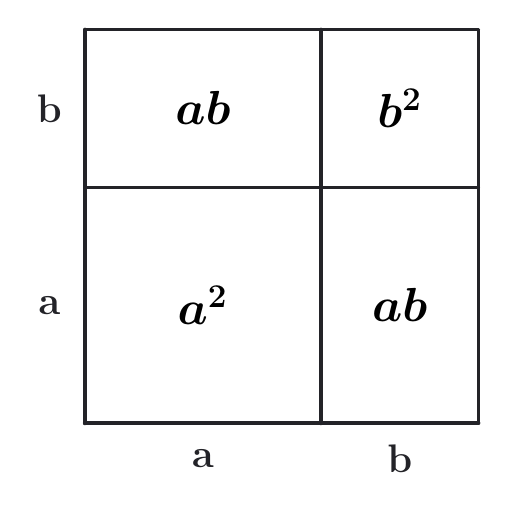
\begin{tikzpicture}[x=1.0000cm,y=1cm,line cap=round,line join=round]
\definecolor{linec0}{RGB}{35,35,40}
\definecolor{linec1}{RGB}{35,35,40}
\definecolor{linec2}{RGB}{35,35,40}
\definecolor{linec3}{RGB}{35,35,40}
\definecolor{linec4}{RGB}{35,35,40}
\definecolor{linec5}{RGB}{35,35,40}
\definecolor{edgecol}{RGB}{35,35,40}
\definecolor{hicol}{RGB}{35,35,40}
\definecolor{angcol}{RGB}{35,35,40}
\coordinate (A) at (0.0000,0.0000);
\coordinate (E) at (3.0000,0.0000);
\coordinate (B) at (5.0000,0.0000);
\coordinate (H) at (5.0000,3.0000);
\coordinate (C) at (5.0000,5.0000);
\coordinate (F) at (3.0000,5.0000);
\coordinate (D) at (0.0000,5.0000);
\coordinate (G) at (0.0000,3.0000);
\draw[line width=1.4pt,color={rgb,255:red,35;green,35;blue,40}] (A) -- (E);
\draw[line width=1.4pt,color={rgb,255:red,35;green,35;blue,40}] (E) -- (B);
\draw[edgecol,line width=1.1pt] (B) -- (H);
\draw[edgecol,line width=1.1pt] (H) -- (C);
\draw[edgecol,line width=1.1pt] (C) -- (F);
\draw[edgecol,line width=1.1pt] (F) -- (D);
\draw[line width=1.4pt,color={rgb,255:red,35;green,35;blue,40}] (D) -- (G);
\draw[line width=1.4pt,color={rgb,255:red,35;green,35;blue,40}] (G) -- (A);
\draw[line width=1.4pt,color={rgb,255:red,35;green,35;blue,40}] (E) -- (F);
\draw[edgecol,line width=1.1pt] (G) -- (H);
\node[font=\bfseries\Large,text={rgb,255:red,35;green,35;blue,40}] at (1.500,-0.450) {a};
\node[font=\bfseries\Large,text={rgb,255:red,35;green,35;blue,40}] at (4.000,-0.450) {b};
\node[font=\bfseries\Large,text={rgb,255:red,35;green,35;blue,40}] at (-0.450,1.500) {a};
\node[font=\bfseries\Large,text={rgb,255:red,35;green,35;blue,40}] at (-0.450,4.000) {b};
\node[fill=white,inner sep=3pt,font=\LARGE,text=black] at (1.500,1.500) {{\boldmath $a^2$}};
\node[fill=white,inner sep=3pt,font=\LARGE,text=black] at (4.000,1.500) {{\boldmath $ab$}};
\node[fill=white,inner sep=3pt,font=\LARGE,text=black] at (1.500,4.000) {{\boldmath $ab$}};
\node[fill=white,inner sep=3pt,font=\LARGE,text=black] at (4.000,4.000) {{\boldmath $b^2$}};
\end{tikzpicture}
\end{document}
